% !TEX root = main.tex
% =============================================================================
% Experiments
% =============================================================================

\section{Experiments}
\label{sec:experiments}

We evaluate the hybrid refine on a synthetic multi-group suite with capsule
clearance.
The goal is to check that the method is usable at scale: hard clearance accept,
dimensionless bend $\kappa r\lesssim 1$, and a clearly decreasing soft objective.

\subsection{Setup}
\label{sec:exp:setup}

\paragraph{Instances.}
We use $N{=}50$ instances from \texttt{hard\_r2}: each is a $48^3$ grid layout
from the companion discrete router~\cite{deng2025pipe_design}
(\textsc{PlaneSlice} corridors + \textsc{PillarField} obstacles), with
\textbf{8 groups}, \textbf{8 terminals per group}, and uniform tube radius
$r{=}2$.
Coarse paths and declared usages are fixed inputs; the refine does not replan
topology.

\paragraph{Protocol.}
All runs use capsule clearance, Chamfer junction union, and the costs of
Sec.~\ref{sec:costs}.
Free Hermite DOF are updated for a budget of $1500$ first-order steps
(Alg.~\ref{alg:refine}) with step size $0.01$, soft clearance margin $0.15$,
and proximity-pair refresh every $10$ steps.
Weights are
$\alpha{=}1$, $\beta{=}1$, $\mu_{\mathrm{obs}}{=}1$, $\mu_{\mathrm{grp}}{=}1$,
$\lambda{=}0.1$, $\eta{=}10$.

\paragraph{Metrics.}
\begin{itemize}
  \item \textbf{Success:} fraction of instances with hard hit count
        $n_{\mathrm{hit}}=0$ (obstacle and cross-group; no soft margin).
  \item \textbf{Path:} aggregate true polyline length $L$, max dimensionless
        bend $\kappa r_{\max}$, and voxel tube volume $V$ (accepted runs).
  \item \textbf{Solve:} wall time, final soft objective $J_T$, and relative drop
        $(J_0-J_T)/J_0$.
\end{itemize}

\subsection{Results}
\label{sec:exp:results}

Table~\ref{tab:exp-main} reports the batch.
All $50$ instances are accepted.
Mean $\kappa r_{\max}\approx 0.97$ stays below one, and the soft objective drops
by about $95\%$ on average
($J_0\!\sim\!6.55\times 10^{3}\!\to\!J_T\!\sim\!3.60\times 10^{2}$).
Mean wall time is about $160\,\mathrm{s}$ per instance under this protocol.

\begin{table}[H]
  \centering
  \caption{Hard\_r2 refine with capsule clearance ($N{=}50$).
  Means over all runs (all accepted).}
  \label{tab:exp-main}
  \begin{tabular}{@{}ccccccc@{}}
    \toprule
    Success & Time (s) & $J_T$ & Rel.\ drop & $L$ & $\kappa r_{\max}$ & $V$ \\
    \midrule
    $50/50$ & $160$ & $360$ & $0.95$ & $4298$ & $0.97$ & $1.91{\times}10^{4}$ \\
    \bottomrule
  \end{tabular}
\end{table}

Fig.~\ref{fig:exp-all} shows the full multi-group packing of instance~0
before and after refine (colors mark groups; obstacles omitted for clarity).
Fig.~\ref{fig:exp-pair} isolates one group so that grid corners vs.\ fair
Hermite tubes are easier to read.
Fig.~\ref{fig:exp-J} plots the soft objective for that run; $J$ drops sharply
in the first few hundred steps and then plateaus.

\begin{figure}[H]
  \centering
  \begin{minipage}[t]{0.495\linewidth}
    \centering
    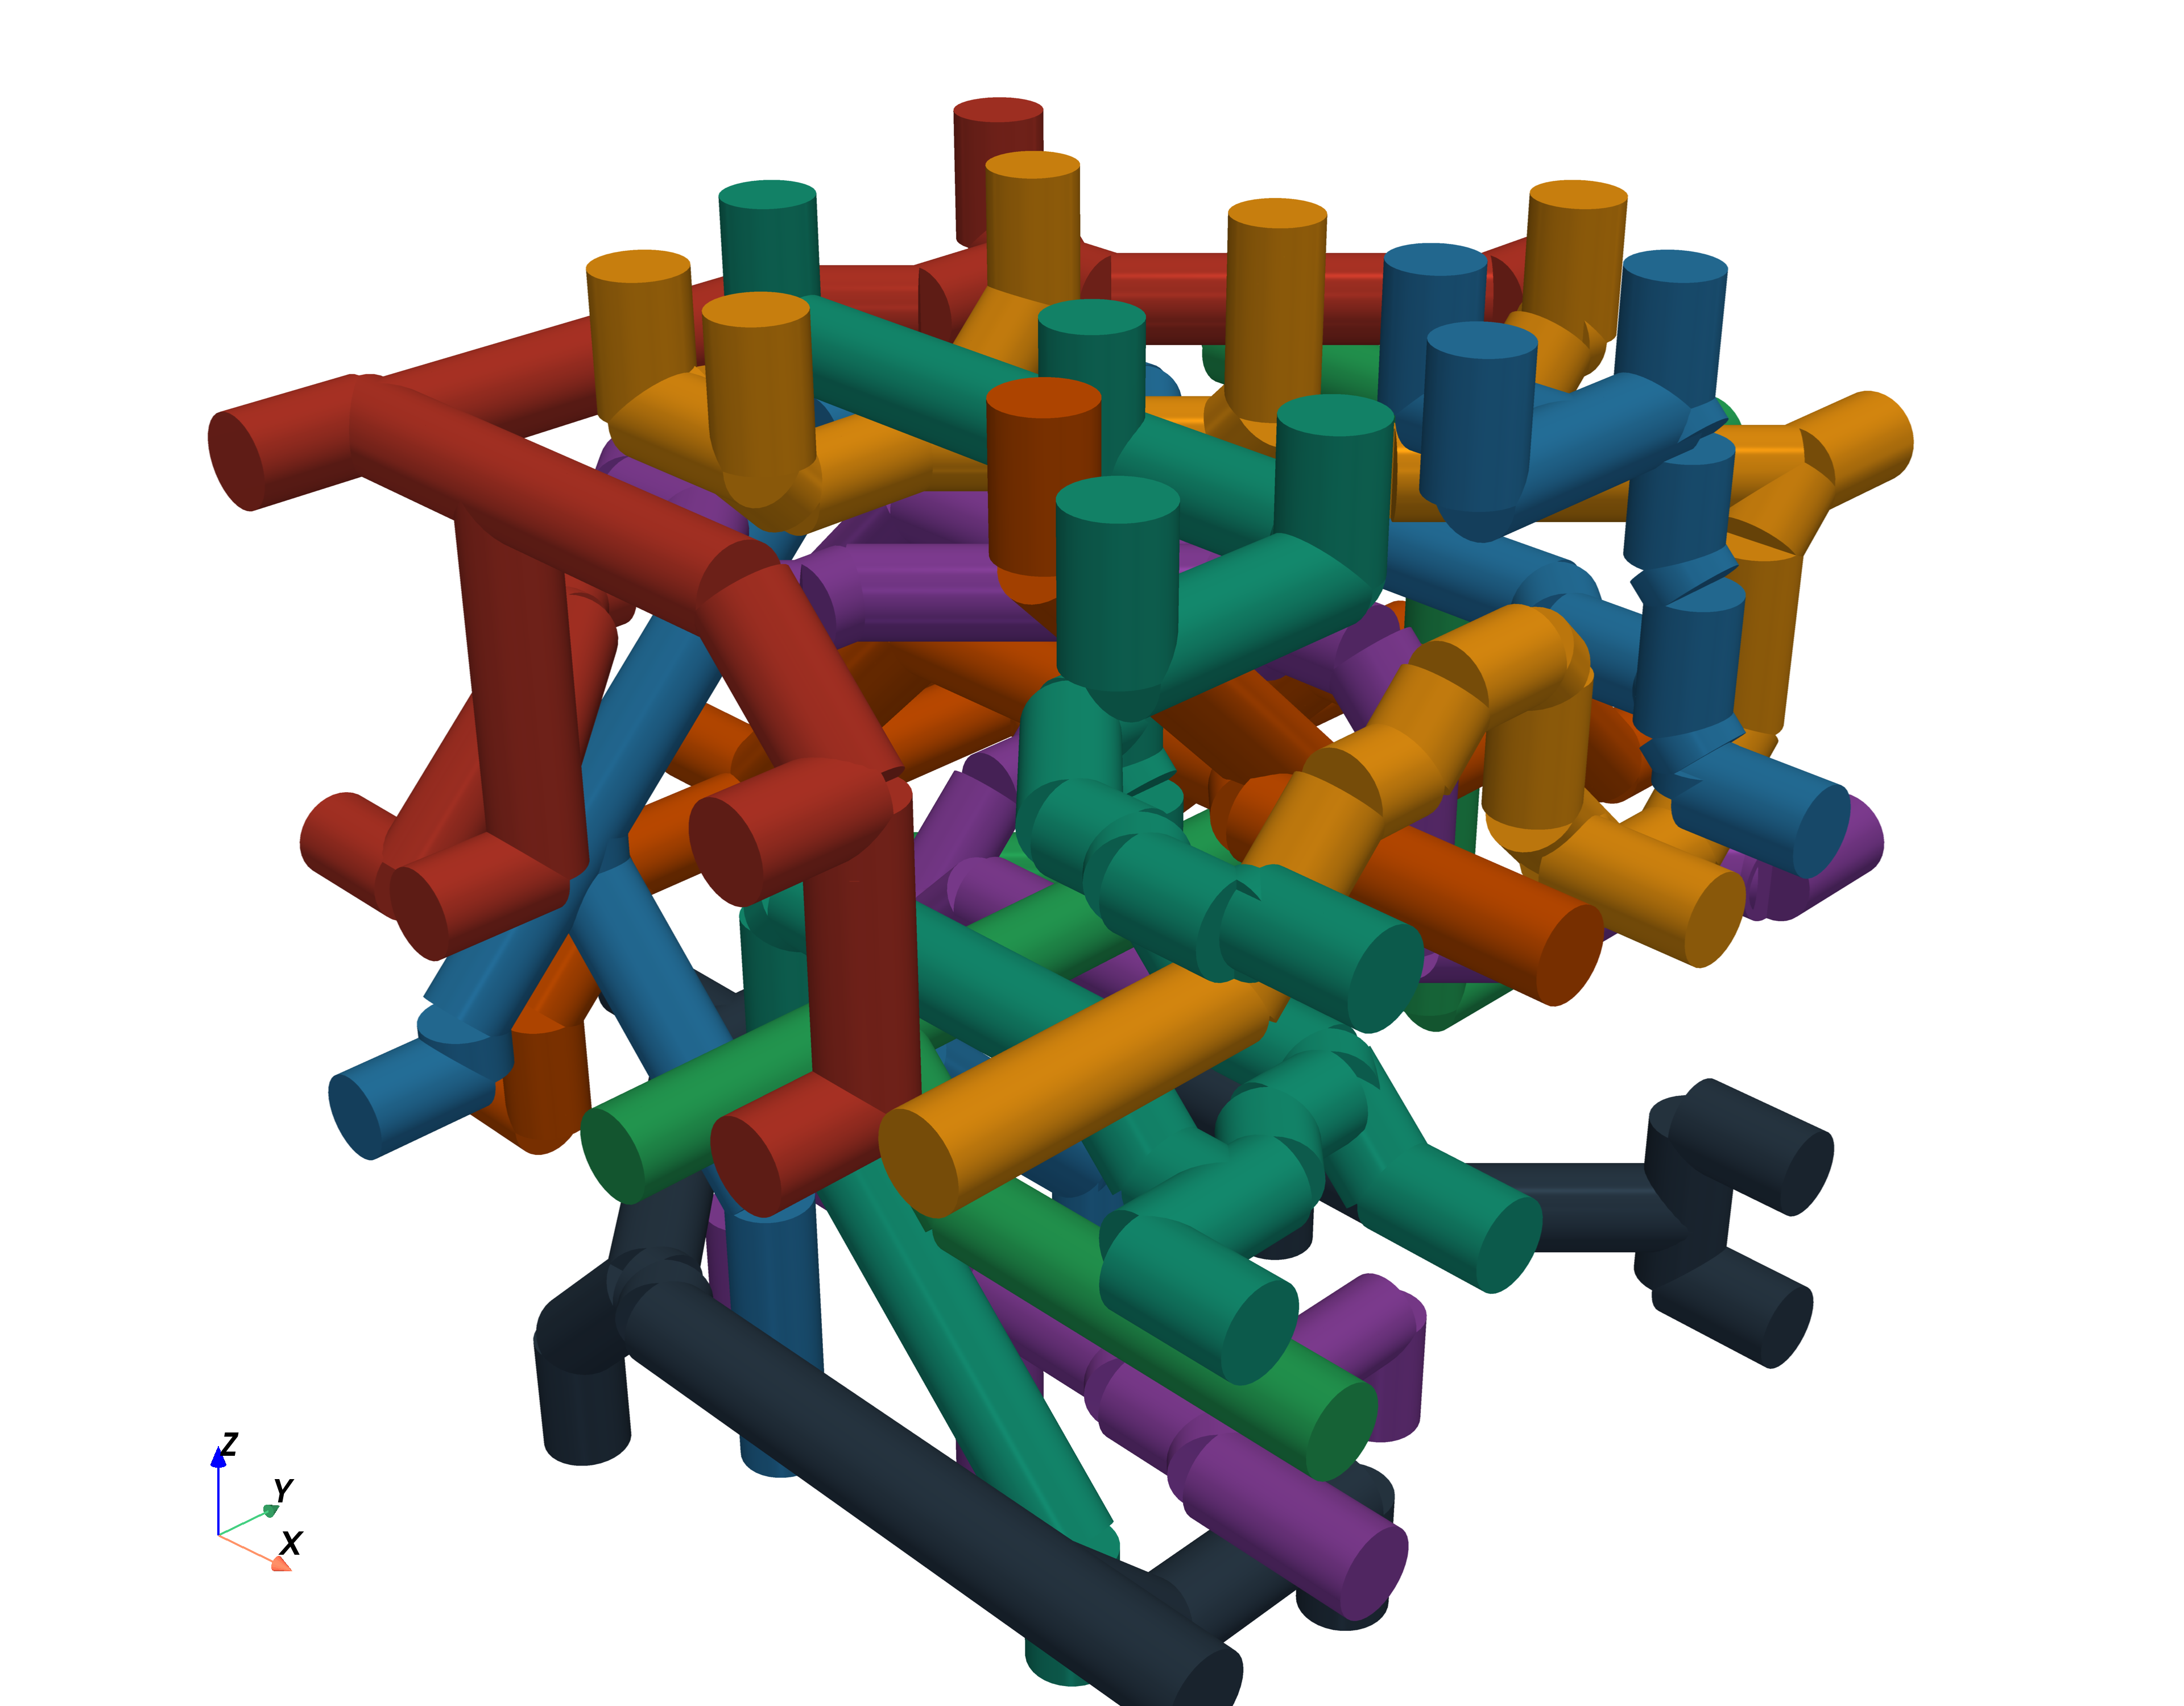
\includegraphics[width=\linewidth]{figures/hard_r2_w1_instance_0_before.png}\\[0.35em]
    {\small Before (coarse)}
  \end{minipage}\hfill
  \begin{minipage}[t]{0.495\linewidth}
    \centering
    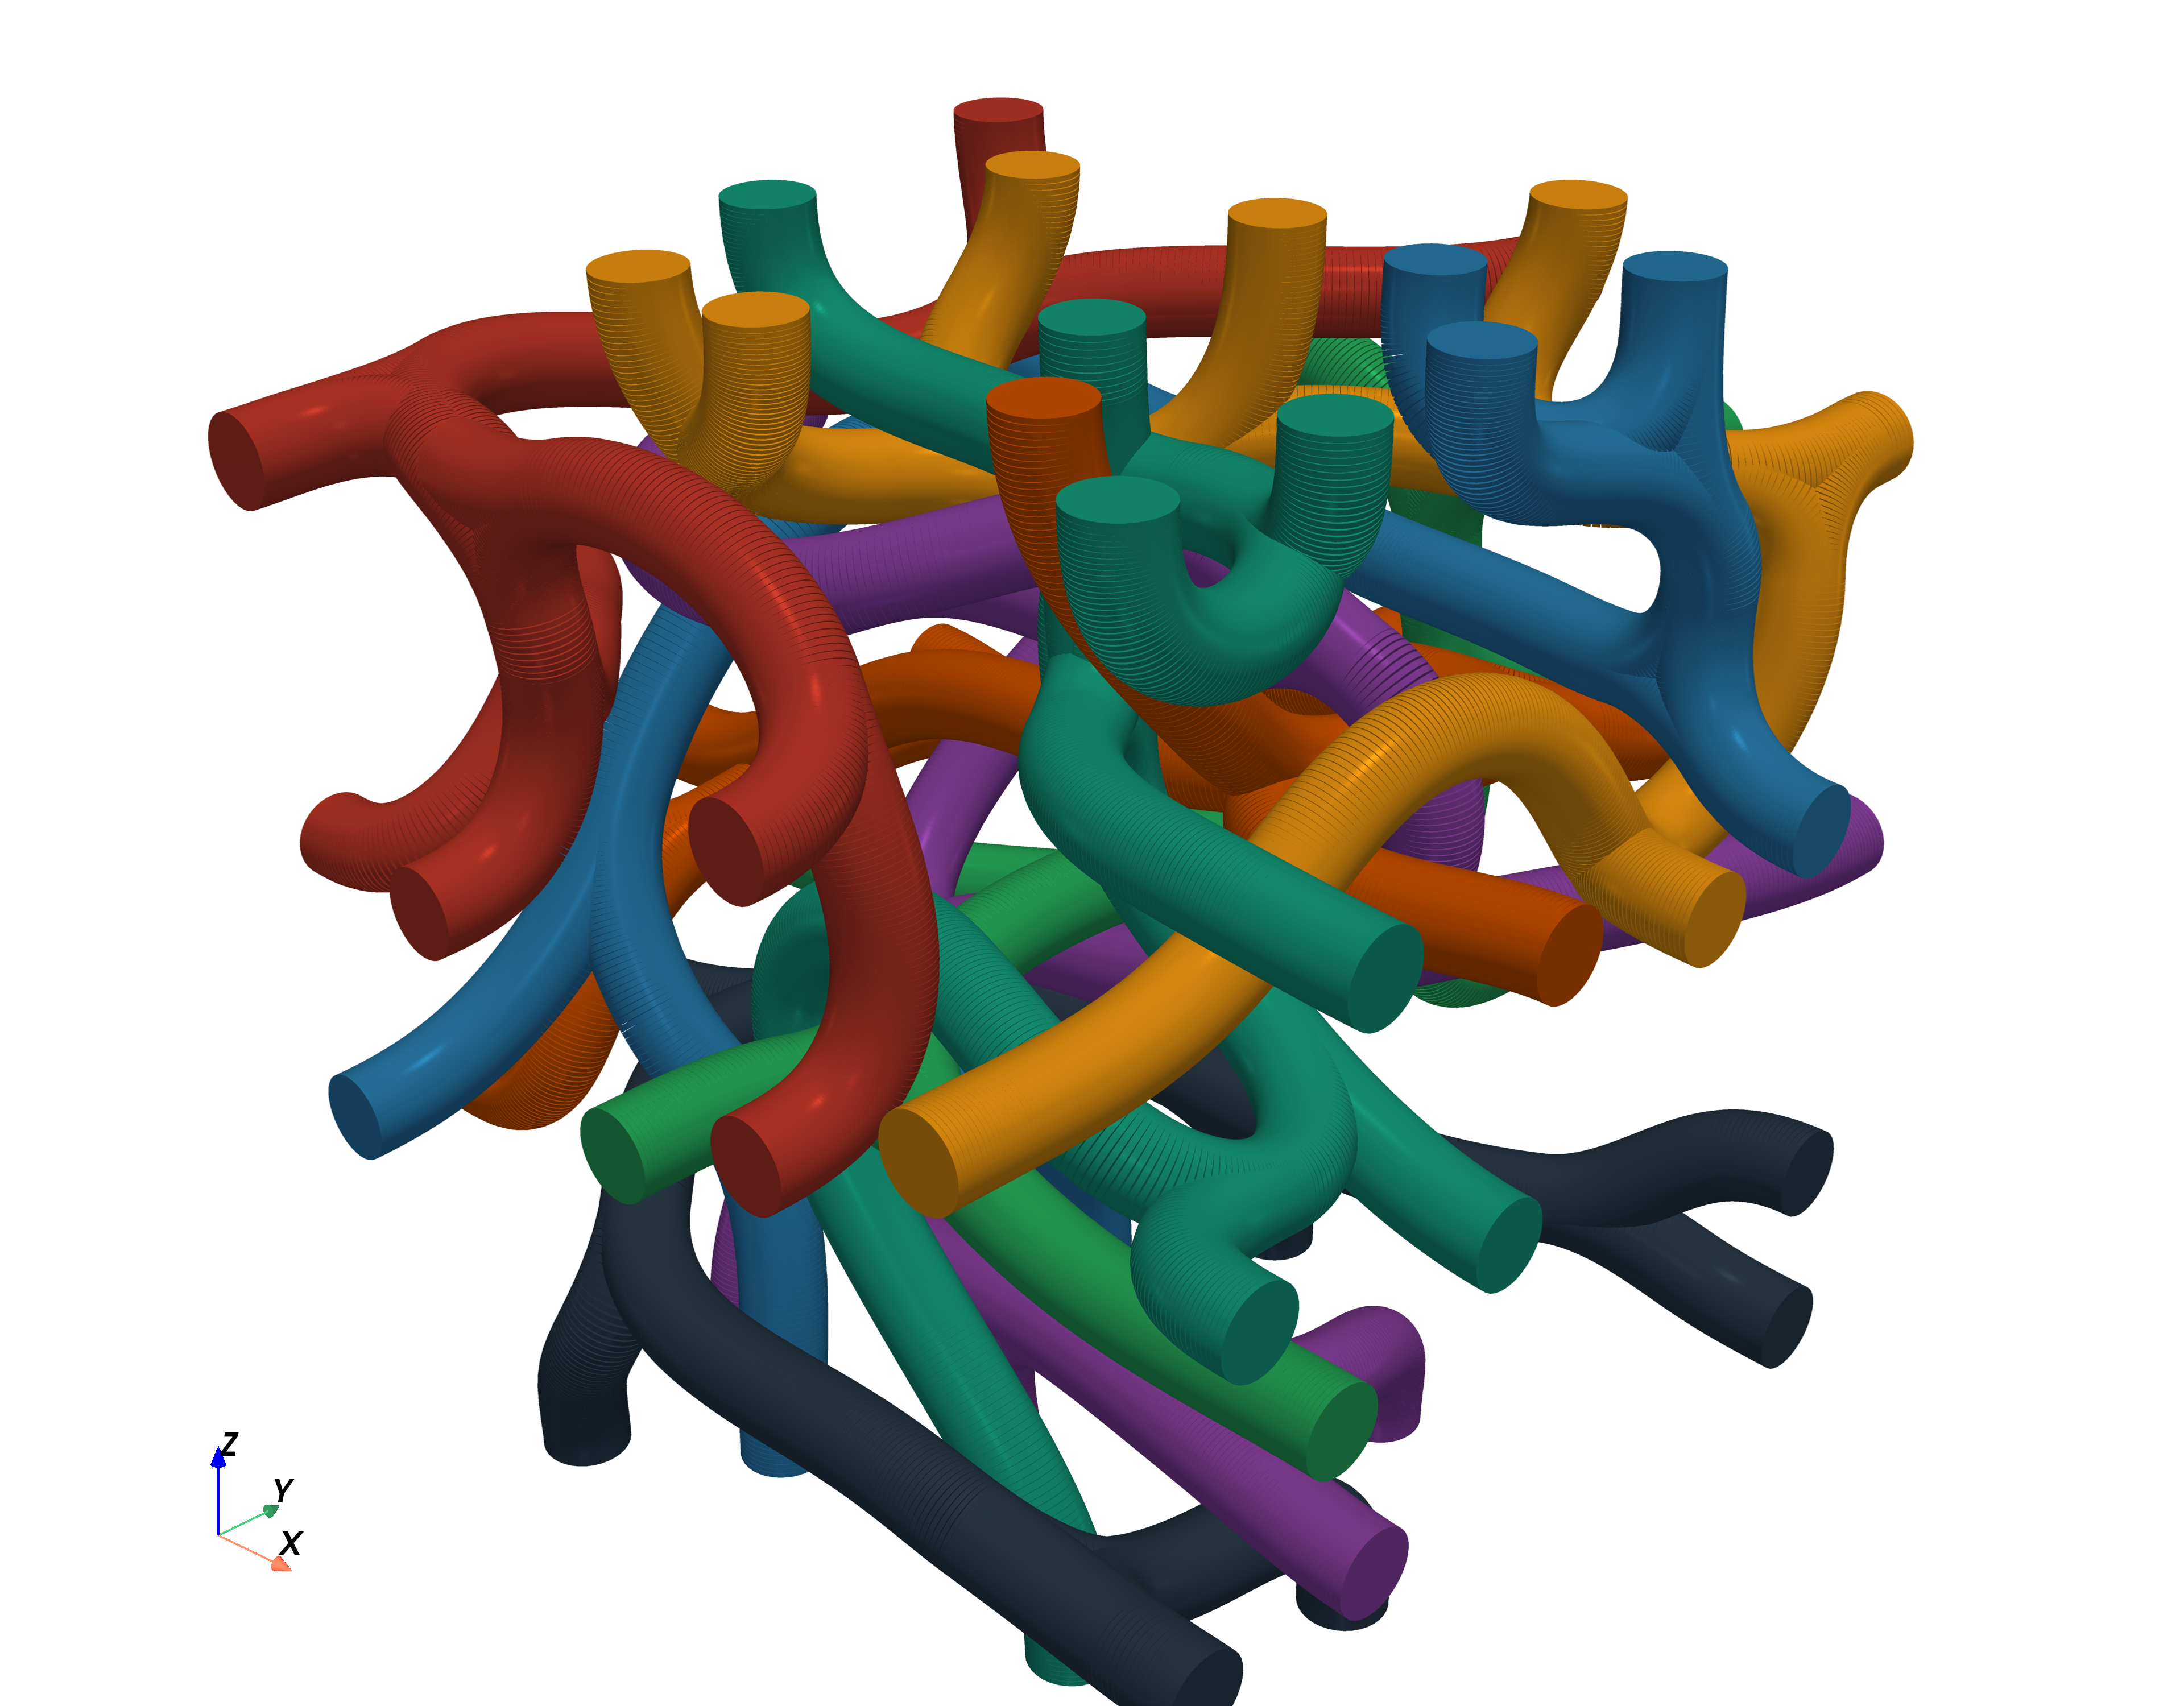
\includegraphics[width=\linewidth]{figures/hard_r2_w1_instance_0_after.png}\\[0.35em]
    {\small After (refined)}
  \end{minipage}
  \caption{All groups of instance~0 from \texttt{hard\_r2}: coarse discrete
  paths (left) vs.\ refined Hermite tubes (right). Colors mark groups;
  obstacles omitted.}
  \label{fig:exp-all}
\end{figure}

\begin{figure}[H]
  \centering
  \begin{minipage}[t]{0.495\linewidth}
    \centering
    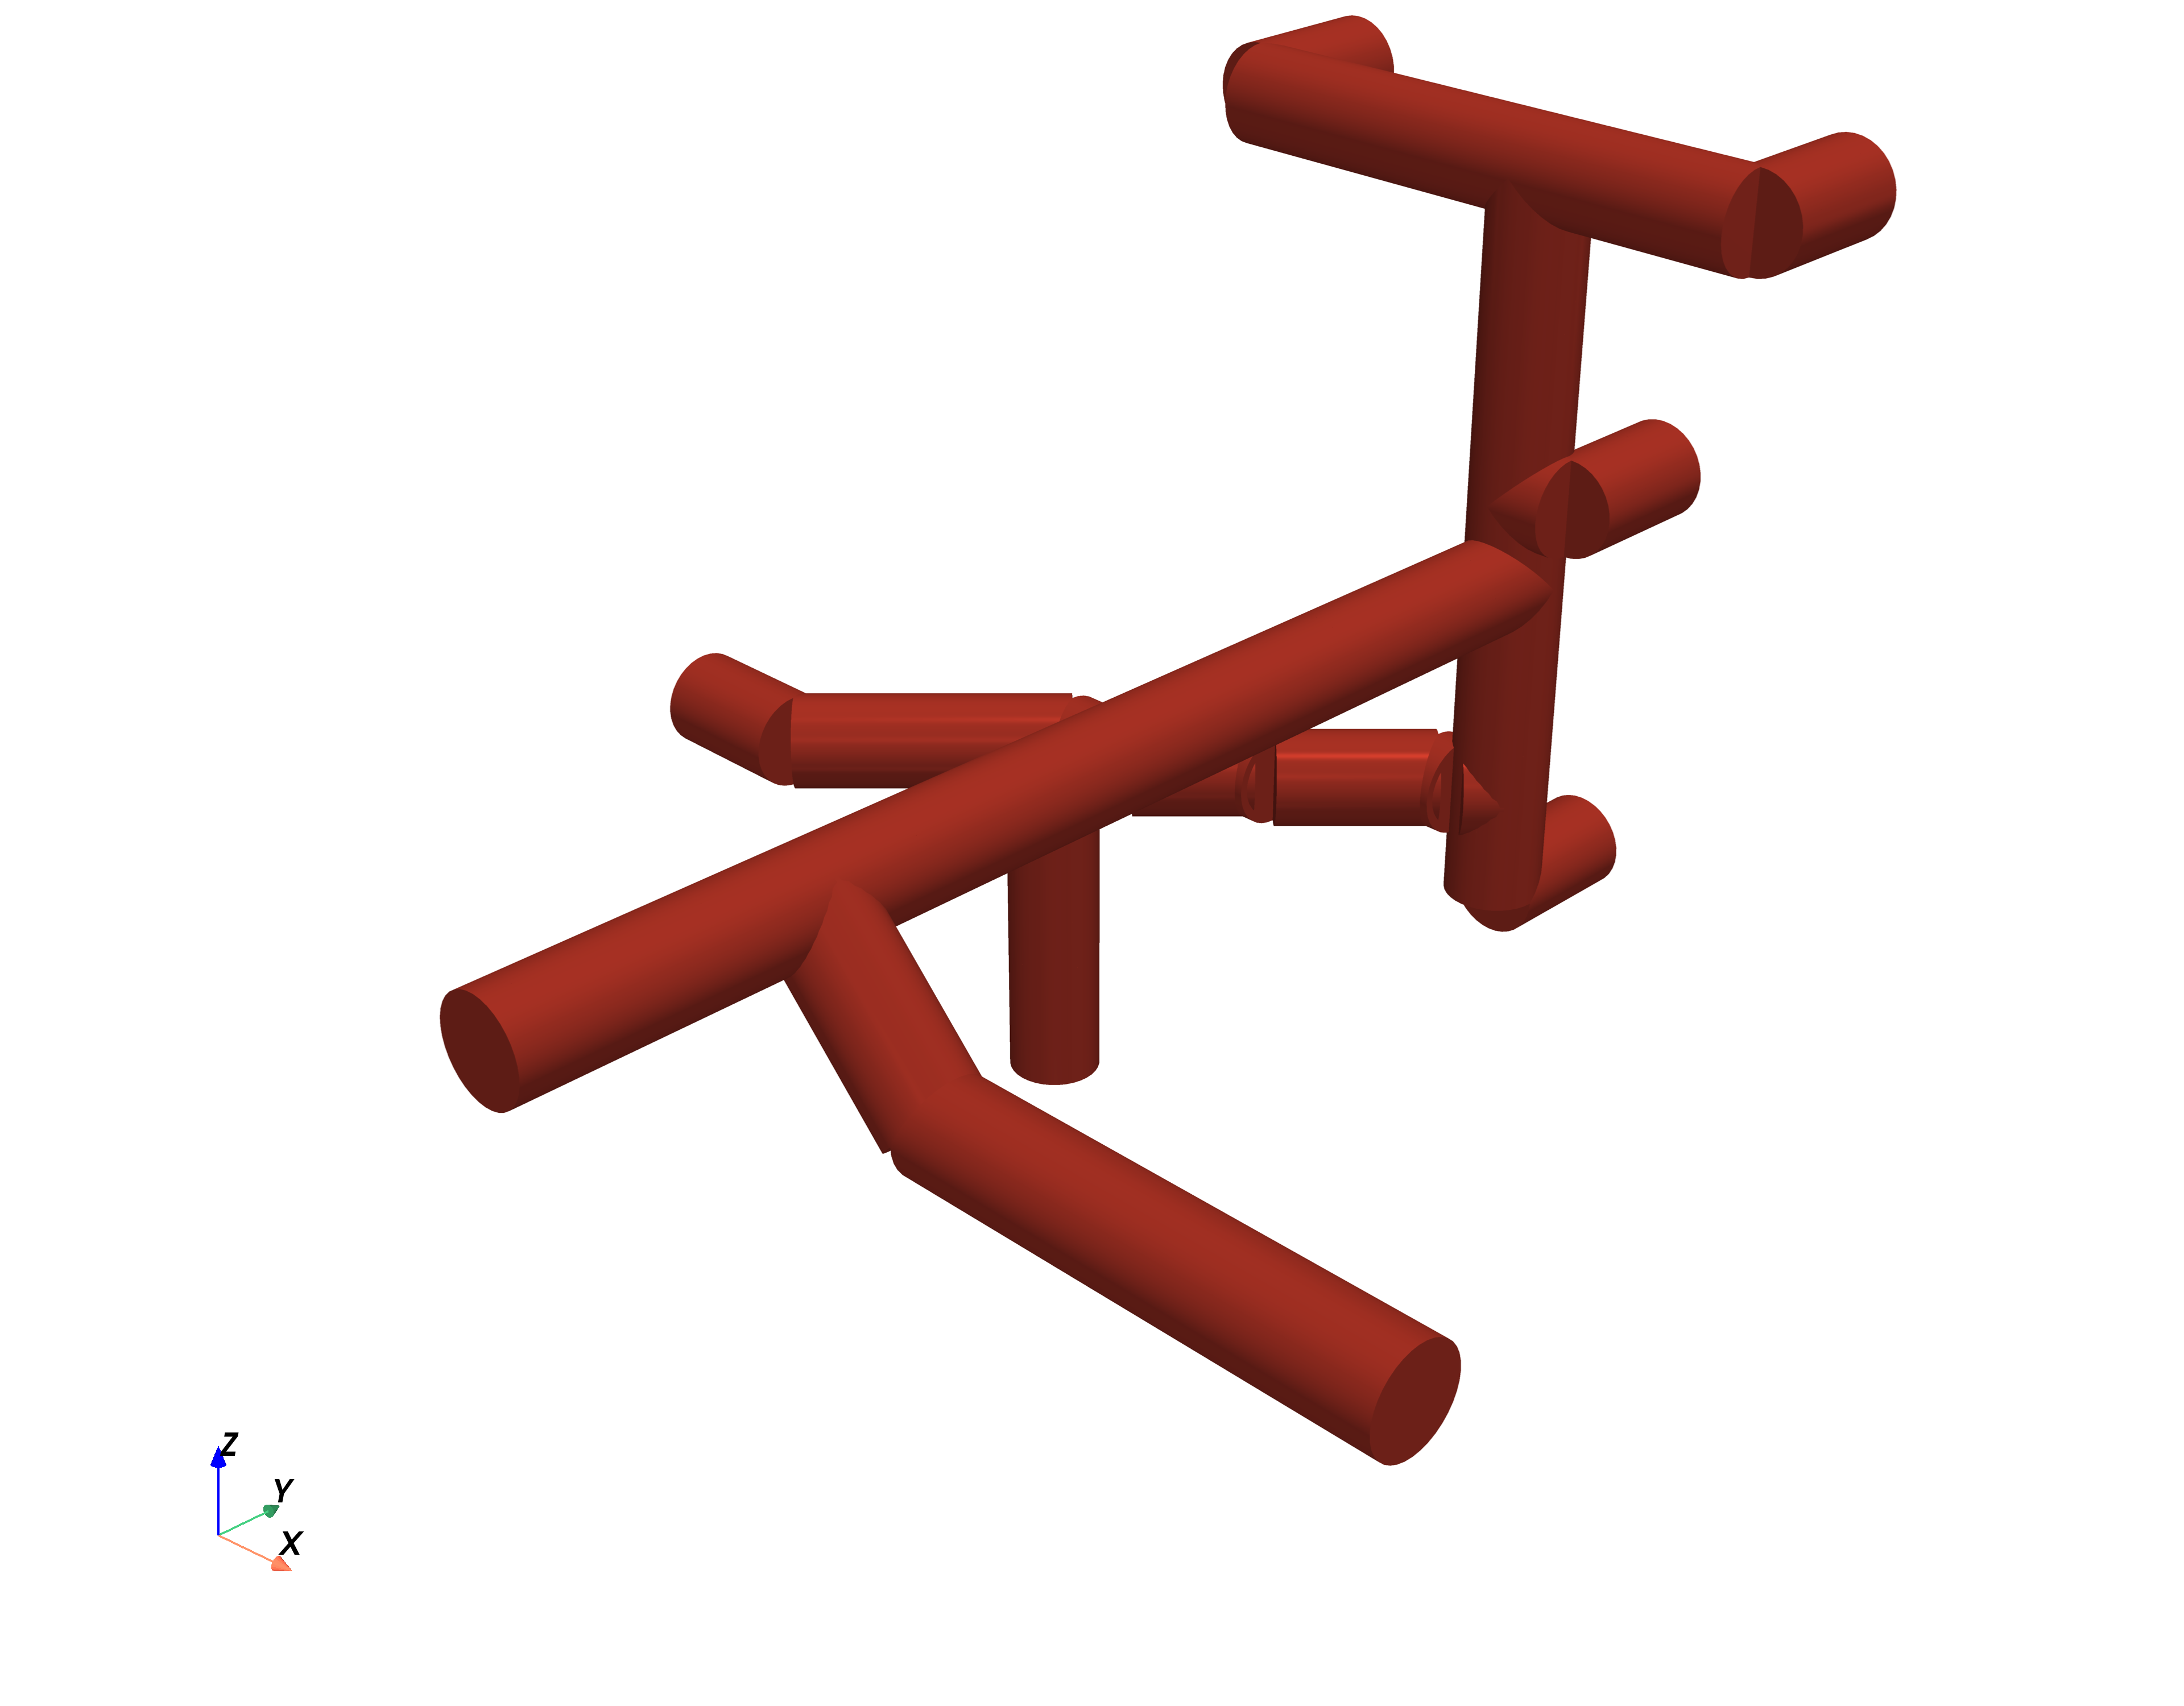
\includegraphics[width=\linewidth]{figures/hard_r2_w1_instance_0_g2_before.png}\\[0.35em]
    {\small Before (coarse)}
  \end{minipage}\hfill
  \begin{minipage}[t]{0.495\linewidth}
    \centering
    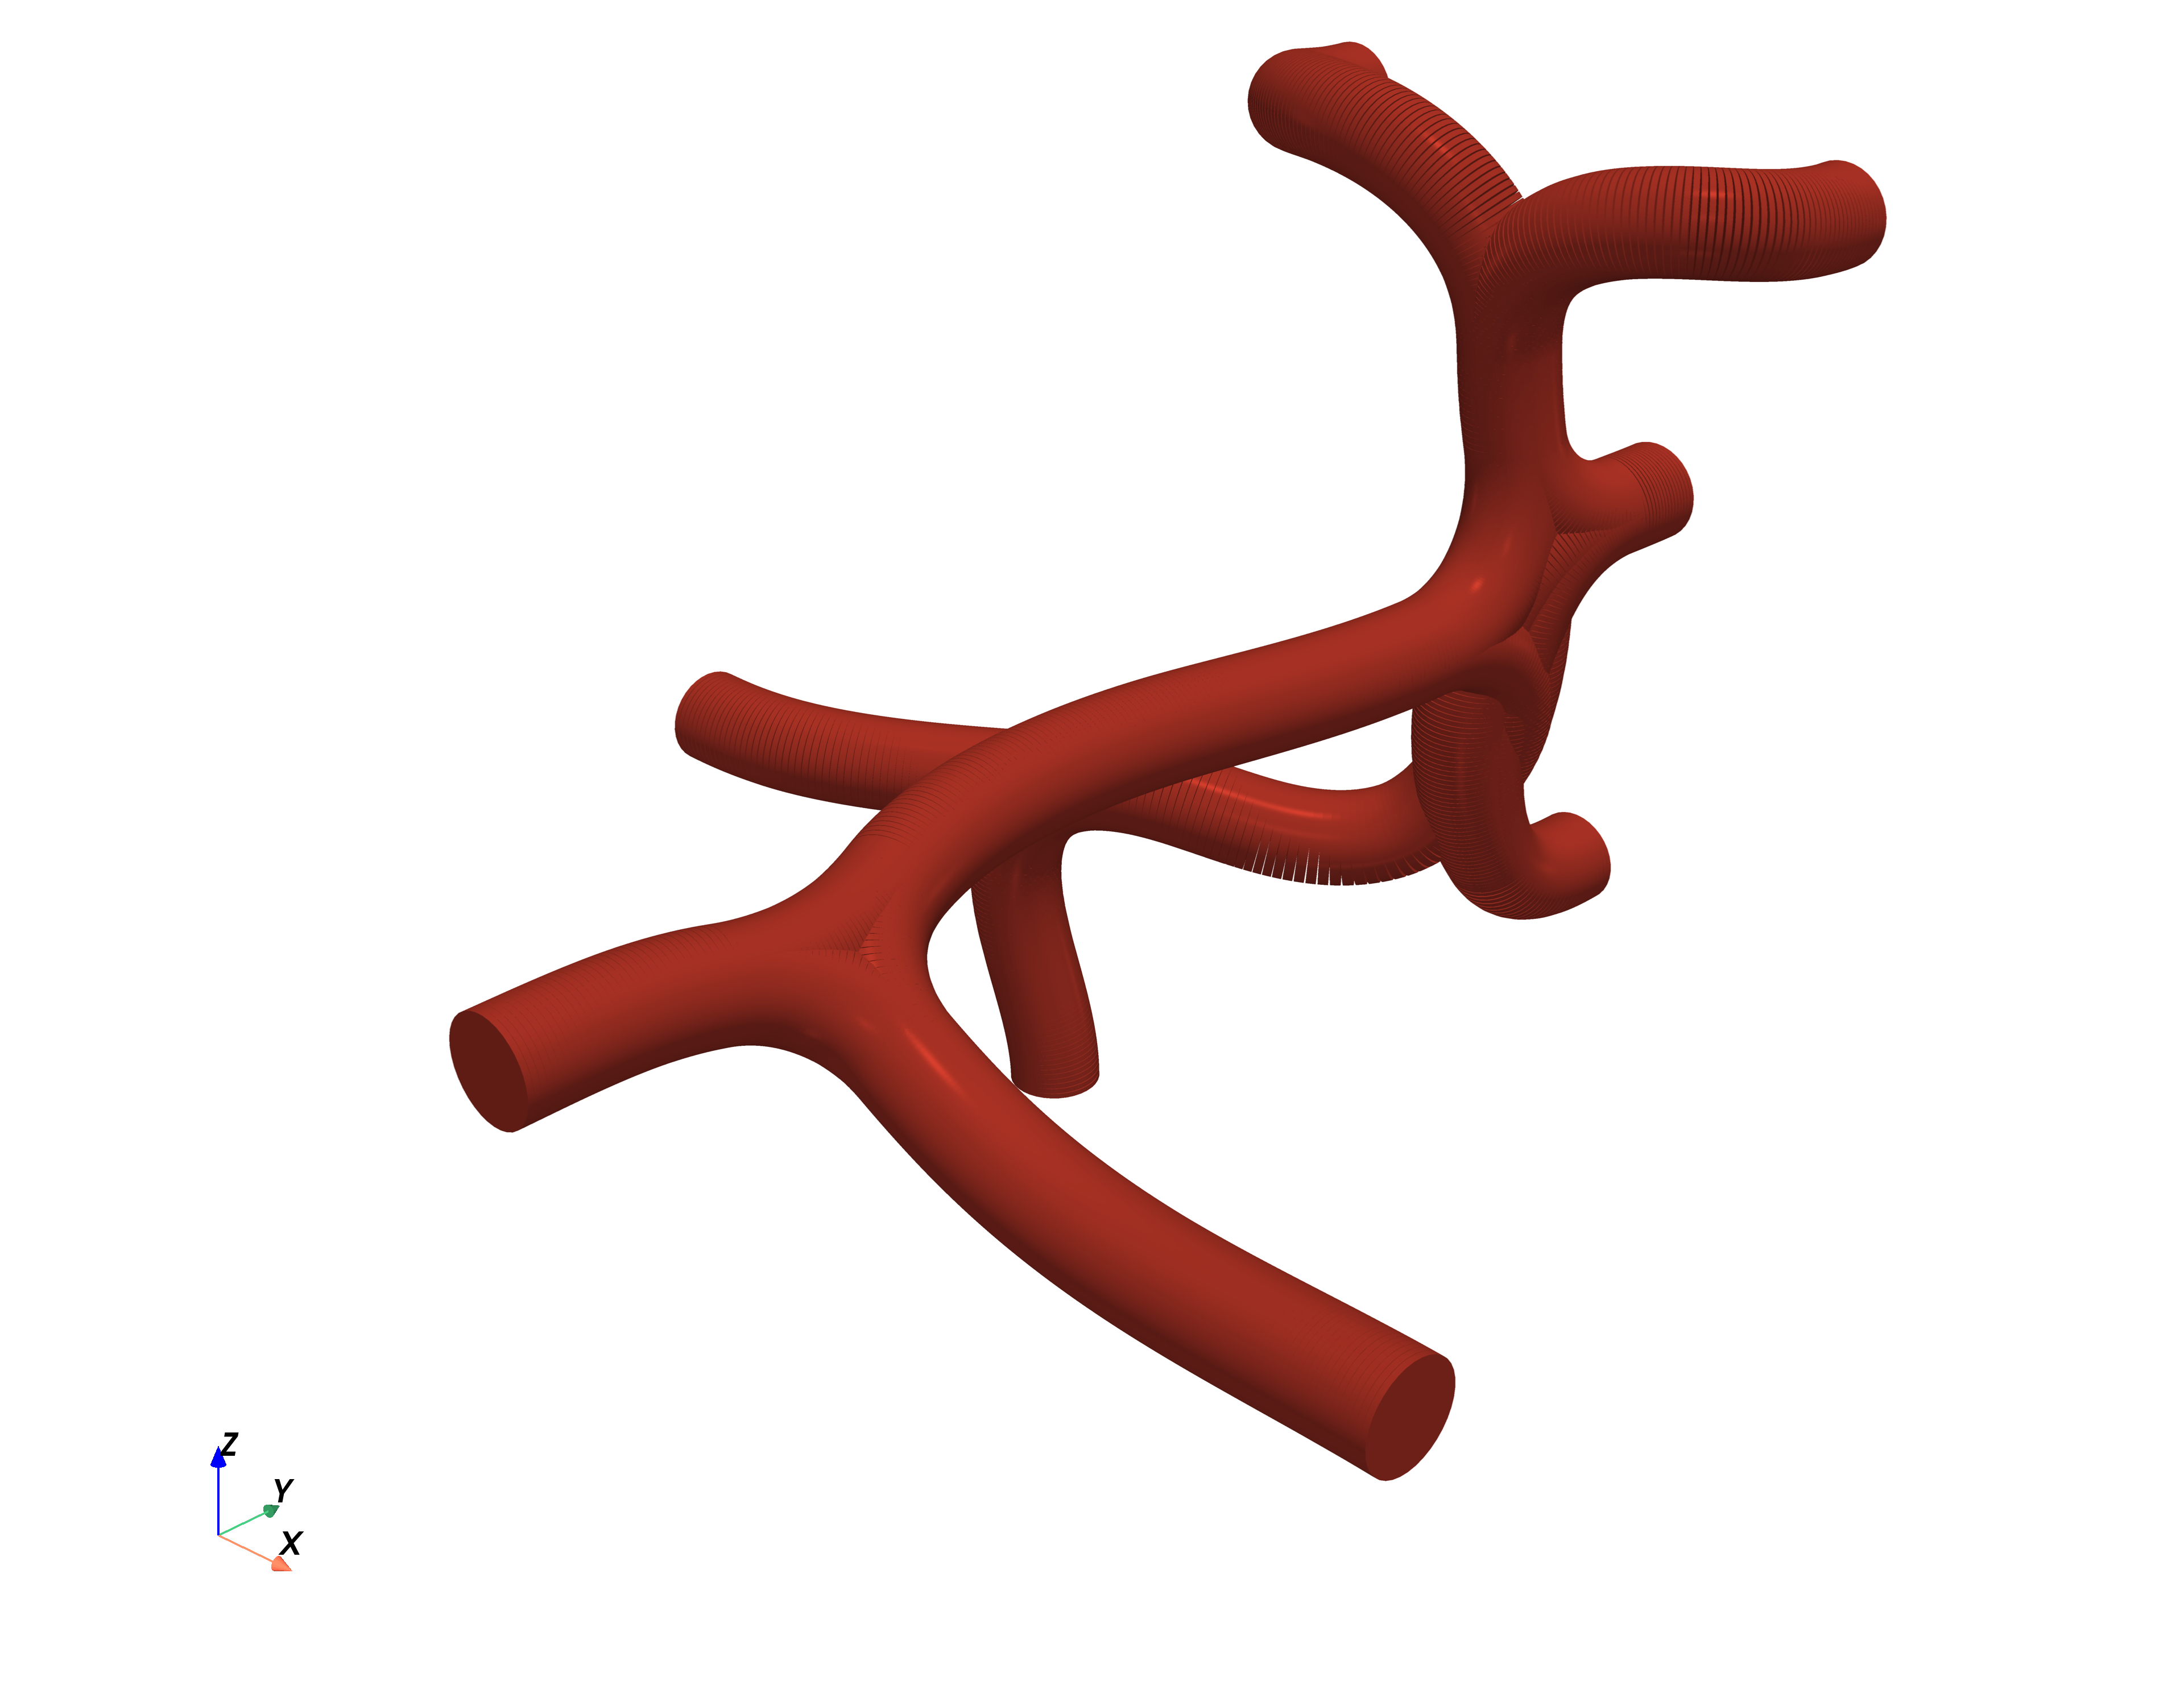
\includegraphics[width=\linewidth]{figures/hard_r2_w1_instance_0_g2_after.png}\\[0.35em]
    {\small After (refined)}
  \end{minipage}
  \caption{Single group ($g_2$) of the same instance, obstacles omitted:
  coarse discrete paths (left) vs.\ refined Hermite tubes (right).}
  \label{fig:exp-pair}
\end{figure}

\begin{figure}[H]
  \centering
  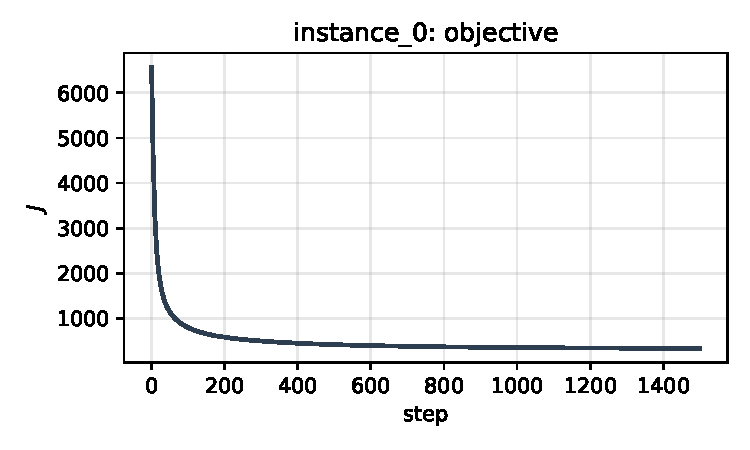
\includegraphics[width=0.72\linewidth]{figures/hard_r2_w1_instance_0_J.pdf}
  \caption{Soft objective $J$ vs.\ iteration for instance~0
  (\texttt{hard\_r2\_w1} / Adam / capsule).}
  \label{fig:exp-J}
\end{figure}

